\documentclass[]{article}
\usepackage[backend=biber, style=numeric]{biblatex}
\usepackage{paralist}
\usepackage{hyperref}
\usepackage{graphicx}
\graphicspath{ {./images/} }

\addbibresource{researchProposal.bib}

%opening
\title{
	A YOLOv8-based Analysis of Image Augmentation Techniques for Vehicle Detection in Adverse Weather Conditions}
	\author{
		Alexander Van Hecke \small(852631385) \and 
		Frederik Lefever    \small(838836963)}

\begin{document}

\maketitle

\begin{abstract}
To do
\end{abstract}

\section{Introduction}

	Adverse weather conditions such as rainfall and snow are widely considered to have an effect on traffic flow. Traffic breakdown occurs when demand exceeds capacity in some part of a transportation network and in \cite{stralenInfluenceAdverseWeather2015} it is shown that the odds of traffic breakdown at bottleneck locations are significantly increased by rainfall. The ensuing economic damage is considerable and provides a strong incentive to mitigate this problem as much as possible. 
	
	Part of a mitigation strategy are traffic monitoring and dynamic flow control. The current technology behind traffic monitoring depends essentially on vehicle detection in images. Yet in turn, vehicle detection in images is itself not indifferent to weather conditions. 
	
	We propose to investigate the effect of image augmentation on the robustness of YOLO{\small v8}-based vehicle detection models. In particular, we propose to investigate the effect of artificially adding rain, fog and snow to real clear weather images of moterways. In comparison with the standard YOLO{\small v8} model, we expect to see an improvement of the Mean Average Precision (mAP) for vehicle detection in models derived from YOLO{\small v8} by training on the augmented images.
	
	The immediate relevance of our findings can be explained in terms of the above mentioned applications to traffic monitoring. But it is not unlikely that some results could be of value to other weather-sensitive arenas, such as surveilance of skiers on mountain slopes.

\section{Literature review}

	In the context of machine learning, image augmentation can broadly be defined as the automated creation of variation in actual image sets. This technique can be used to avoid a learning algorithm overfitting the data. Overfitting occurs when a learning algorithm learns a function in such a way that it perfectly models the training data. Large volumes of data with sufficient variation can alleviate the problem of overfitting. Yet sometimes sampling data from an application domain is nontrivial, eg. when learning from medical images. 
	
	A comprehensive survey of modern image augmentation techniques is presented in \cite{shortenSurveyImageData2019}. Several approaches such as geometric transformations, color space augmentations, kernel filters, mixing images, random erasing, feature space augmentation, adversarial training, generative adversarial networks, neural style transfer, and meta-learning, are treated with mild technicality. \cite{xuComprehensiveSurveyImage2023} offers a more recent survey of image augmentation techniques as used in deep learning. This survey introduces a novel taxonomy, where image augmentation algorithms are classified as either model-free, modelbased, or optimizing policy-based. The objectives of image augmentation are explained from an analysis of challenges encountered when deploying deep learning models for computer vision. A theoretical framework for understanding data augmentation is described in \cite{daoKernelTheoryModern2019}. First a general model of augmentation as a Markov process is provided, and it is shown that kernels appear naturally with respect to this model. Next, a more directly analysis of the effect of augmentation on kernel classifiers is offered.
	
	The effectiveness of image augmentation on the classification of images with deep learning is discussed in \cite{perezEffectivenessDataAugmentation2017}. Simple techniques, such as cropping,	rotating, and flipping images are compared. Additionally this paper reports on experiments with generative adversarial neural networks to learn augmentation strategies. 
	
	Research similar to the proposed research can be found in \cite{kumarObjectDetectionAdverse2023}. The central question in \cite{kumarObjectDetectionAdverse2023} is whether YOLO{\small v8} can be improved through transfer learning to detect objects in adverse weather. This paper supports the hypothesis that training with actual images of adverse weather conditions significantly improves the detection performance compared to the standard YOLO{\small v8} model. An enhanced YOLO-based model for vehicle detection in foggy weather conditions is the focus of \cite{liVehicleDetectionFoggy2022}. The approach used to create the enhanced model is interesting in that the trainingset is obtained from 350 traffic images that are augmented with a fog-effect and subsequently dehazed with the multi-scale retinex with color restoration (MSRCR) algorithm. The final trainingset is then composed of the original images, fogged images and dehazed images. Whereas results in \cite{liVehicleDetectionFoggy2022} are reported with autonomous vehicles in mind, \cite{songVisionbasedVehicleDetection2019} specifically targets vehicle detection and counting in highway management.  A new segmentation method is proposed to divide a depicted highway road surface into a distal and a proximal area. Using this separation a YOLO{\small v3} model is trained to detect the type and location of vehicles. To estimate vehicle count and trajectories the Oriented FAST and Rotated BRIEF (ORB) algorithm is added to the image processing pipeline.
	
	
	
	


	



\section{Research questions}

	The image augmentation techniques described in the literature are numerous and varied, ranging from simple geometric transformations to the addition of noise and the changing of color, saturation and hue parameters. We propose to investigate the effect of thematic image augmentation consisting of the addition of rain, fog and snow to clear weather images. At the more general level, we aim to answer following question:
	
	\textit{Given that the standard YOLO{\small v8} model is used as a comparative baseline and trained with thematically augmented images, will the resulting model then be more accurate in predicting the presence of vehicles in actual images of traffic in adverse weather conditions?}
	
	Furthermore, to appreciate the value of image augmentation in contexts where data is not necessarily scarce, we pose an additional question:
	
	\textit{Given that the standard YOLO{\small v8} model is trained with actual images of traffic in adverse weather conditions, how then does the accuracy of the resulting model compare to the accuracy of a model derived from standard YOLO{\small v8} with augmented images?}
	

\section{Research method}
\subsection{Measuring model accuracy}

	To estimate the robustness of vehicle detection models, we use the mean average precision (mAP) metric. The mAP is an aggregate metric based on the confusion matrix, the intersection over union (IoU), recall and precision. We consider three relevant classes of vehicles, nl. 'car', 'bus' and 'truck'.

\subsubsection{Calculation of the mAP}

	The $mAP$ is calculated by deviding the sum of the average precision ($AP$) per class by the number of classes $N$.
	
	\[
	mAP = \frac{1}{N} \sum_{i=1}^{N} AP_i
	\]
	
	In summary, the $AP$ of a model is obtained by following steps:
	
	\begin{center}
		\begin{compactenum}
			\item Use model to generate prediction scores
			\item Map prediction scores onto class labels
			\item Construct the confusion matrix
			\item Calculate precision and recall for a set of IoU thresholds
			\item Calculate area under precision-recall curve
			\item Calculate average precision
		\end{compactenum}
	\end{center}
	
	The IoU metric is used to evaluate the performance of object detection by quantifying the fit between the ground truth bounding box and the predicted bounding box.
	
	\begin{figure}[h]
		\centering
		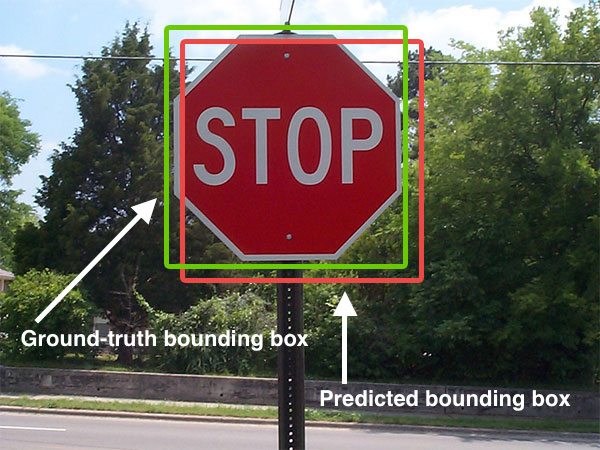
\includegraphics[width=5cm]{Intersection_over_Union_-_object_detection_bounding_boxes.jpg}
		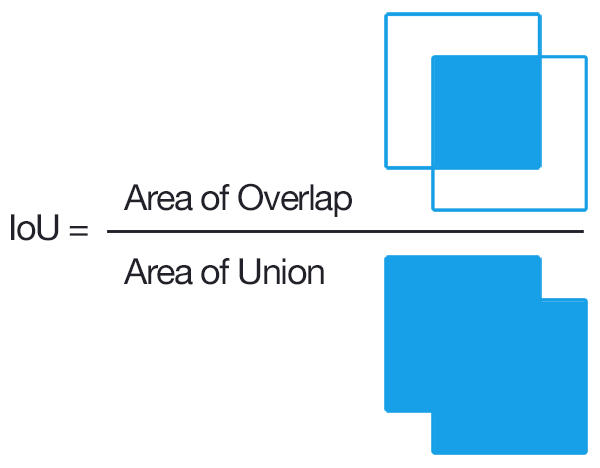
\includegraphics[width=5cm]{Intersection_over_Union_-_visual_equation.png}
		\caption{Images from Wikipedia \footnotesize{(\url{https://en.wikipedia.org/wiki/Jaccard_index})}}
	\end{figure}
	
	By using a lower bound for the value of the IoU metric, one can discriminate between positive and negative predictions. The IoU metric can then be used to calculate recall and precision. In the context of traffic management, it seems reasonable to slightly favour recall over precision and choose an IoU threshold to reflect this preference. However, choosing a good IoU threshold is itself an optimization process. For comparing models, optimizing the IoU threshold is unnecessary. Instead, we calculate AP as an average of AP's calculated for a set of IoU thresholds per class.

\subsection{Data collection}

	Two open-source datasets are used for this research. The DAWN dataset \cite{bw1x-yh39-20} is a collection of 1000 images from real-traffic environments in adverse weather conditions. The images are divided into four sets of weather conditions: fog, snow, rain and sandstorms. They are labelled according to the categories relevant for current research (``car'', ``bus'', ``truck'') and annotated with object bounding boxes. We use the DAWN dataset for both validation and training. 
	
	The second dataset is the UA-DETRAC \cite{CVIU_UA-DETRAC} dataset. This dataset provides 140K traffic images taken at Beijing and Tianjin (China). Images of the UA-DETRAC dataset are divided into four weather categories: ``cloudy'', ``night'', ``sunny'' and ``rainy''. They are labelled ``car'', ``bus'', ``van'' and ``others''; and object bounding boxes are provided. The dataset is made available as a bi-partition (DETRAC-Train-Images and DETRAC-Test-Images). From the union of the train and test datasets, we only use images of the category ``sunny'' for data augmentation and training. No other images are used from the UA-DETRAC dataset.

\subsection{Model selection}
 
	For vehicle detection we chose an open source convolutional neural network called YOLO{\small v8} \cite{yolov8_ultralytics}. We use this model in transfer learning and as a reference for derived models. YOLO{\small v8} is trained on the Microsoft COCO dataset \cite{linMicrosoftCOCOCommon2015a} and capable of detecting object categories ``car'', ``bus'' and ``truck''. 
 
\subsection{Experiments}

	Since the chosen augmentation software imgaug \cite{imgaug} (version 0.4.0) lacks the capability to add sandstorm effects to images, we start by creating a subset of the DAWN dataset by excluding all images of the weather category ``sandstorm''. The resulting subset is then randomly partitioned with a 80/20 ratio. The larger part is denoted by DAWN-train and the smaller part by DAWN-test. 
	
	Next we establish a baseline measurement, by presenting the DAWN-test set to the standard YOLO{\small v8} model and determine its mAP over the ``car'', ``bus'' and ``truck'' classes. Then, we compose the union of the DETRAC-Train-Images and DETRAC-Test-Images and from it extract images of the weather category ``sunny''. The extracted images are used to produce three distinct trainingsets by augmenting them with fog, rain and snow using imgaug \cite{imgaug}. The obtained trainingsets are denoted resp. DETRAC-fog, DETRAC-rain and DETRAC-snow. We then train the standard YOLO{\small v8} model with the union of the DETRAC-fog, DETRAC-rain and DETRAC-snow datasets. Finally, we determine the mAP of the new model over the  ``car'', ``bus'' and ``truck'' classes, by presenting it the DAWN-test set. Comparing the mAP of the baseline with the mAP of the new model should provide some ground for answering the first research question.
	
	To answer the second research question, we train the standard YOLO{\small v8} model with the DAWN-train set and measure the mAP of the derived model. Like before, the mAP is calculated over the ``car'', ``bus'' and ``truck'' classes for the DAWN-test set.

\section{Proposed time line}



\printbibliography

\end{document}
